\documentclass[11pt]{article}
\usepackage[a4paper, margin=1in]{geometry}
\usepackage{cite}
\usepackage{amsmath,amssymb,amsfonts}
\usepackage{algorithmic}
\usepackage[export]{adjustbox}
\usepackage{graphicx}
\usepackage{textcomp}
\usepackage{listings}
\usepackage{matlab-prettifier}
\usepackage{tabularx}
\usepackage{longtable}
\usepackage{caption}
\usepackage{pdflscape}
\usepackage{subcaption}
\usepackage{url}
\usepackage{hyperref}
\usepackage{array}
\usepackage{lastpage}
\raggedbottom
\usepackage{cite}
\usepackage{indentfirst}
\usepackage{fancyhdr}
\renewcommand*\contentsname{TABLE OF CONTENTS}
\renewcommand{\listfigurename}{List of Figures}
\begin{document}
\tableofcontents
\listoffigures
\listoftables
\pagestyle{fancy}
\fancyhead{}
\fancyhead[LO,LE]{Name: Md. Raisul Islam Rifat}
\fancyhead[RO,RE]{ID: 1902081}
\fancyfoot{}
\fancyfoot[RE,RO]{Page \thepage\ of \pageref{LastPage}}
\newpage
\section{Abstract}
In this lab, we explored the design and simulation of a CMOS circuit representing the Boolean equation $Y=A\cdot(B+C)\cdot(D+E)$ using Cadence Virtuoso. The objective was to construct a functional schematic that accurately reflects the equation's logic. Through simulation, we analyzed the performance characteristics of the circuit, including logic levels and propagation delay. The results validated the design approach and demonstrated the effectiveness of CMOS technology in implementing complex Boolean functions.
\section{Keywords}
CMOS, VLSI, Boolean algebra, digital logic design, Cadence Virtuoso, circuit simulation, NMOS, PMOS, logic gates, schematic design, circuit implementation, digital circuits.
\section{Objectives}
\begin{enumerate}
    \item To design a CMOS circuit from the given Boolean equation.
    \item To observe the transient response of the designed CMOS circuit.
\end{enumerate}
\section{Introduction}
The integration of digital circuits in modern electronics necessitates efficient design methodologies that leverage complementary metal-oxide-semiconductor (CMOS) technology. CMOS circuits are favored for their low power consumption and high noise immunity. This lab focused on designing a CMOS schematic to implement the specific Boolean function $Y=A\cdot(B+C)\cdot(D+E)$. By utilizing Cadence Virtuoso for simulation, we aimed to visualize the circuit's behavior, validate its functionality, and understand the interplay of logic gates in realizing the intended output. This hands-on experience provided a practical understanding of how Boolean algebra translates into physical circuit designs.
\section{Theory}
The Boolean equation $Y=A\cdot(B+C)\cdot(D+E)$ consists of both AND and OR operations. In this equation:
\begin{itemize}
    \item $A$ is an AND input that controls the output based on its logic level.
    \item $(B+C)$ and $(D+E)$ re OR inputs that contribute to the overall output when combined with $A$.
\end{itemize}
The corresponding CMOS implementation involves using PMOS and NMOS transistors to create the desired logic levels. PMOS transistors are used to pull the output high (logic 1) when the input conditions are met, while NMOS transistors pull the output low (logic 0). The circuit employs a combination of parallel and series connections to reflect the OR and AND operations respectively, allowing for a dynamic response to varying input conditions. Cadence Virtuoso facilitates detailed circuit analysis, providing insights into the electrical characteristics and timing behavior of the designed schematic.
\newpage
\section{Truth table}
\begin{table}[!h]
    \centering
    \begin{tabular}{|l|l|l|l|l|c|}
        \hline
        $A$ & $B$ & $C$ & $D$ & $E$ & $Y=A\cdot(B+C)\cdot(D+E)$ \\ \hline
        0   & 0   & 0   & 0   & 0   & 0                         \\ \hline
        0   & 0   & 0   & 0   & 1   & 0                         \\ \hline
        0   & 0   & 0   & 1   & 0   & 0                         \\ \hline
        0   & 0   & 0   & 1   & 1   & 0                         \\ \hline
        0   & 0   & 1   & 0   & 0   & 0                         \\ \hline
        0   & 0   & 1   & 0   & 1   & 0                         \\ \hline
        0   & 0   & 1   & 1   & 0   & 0                         \\ \hline
        0   & 0   & 1   & 1   & 1   & 0                         \\ \hline
        0   & 1   & 0   & 0   & 0   & 0                         \\ \hline
        0   & 1   & 0   & 0   & 1   & 0                         \\ \hline
        0   & 1   & 0   & 1   & 0   & 0                         \\ \hline
        0   & 1   & 0   & 1   & 1   & 0                         \\ \hline
        0   & 1   & 1   & 0   & 0   & 0                         \\ \hline
        0   & 1   & 1   & 0   & 1   & 0                         \\ \hline
        0   & 1   & 1   & 1   & 0   & 0                         \\ \hline
        0   & 1   & 1   & 1   & 1   & 0                         \\ \hline
        1   & 0   & 0   & 0   & 0   & 0                         \\ \hline
        1   & 0   & 0   & 0   & 1   & 0                         \\ \hline
        1   & 0   & 0   & 1   & 0   & 0                         \\ \hline
        1   & 0   & 0   & 1   & 1   & 0                         \\ \hline
        1   & 0   & 1   & 0   & 0   & 0                         \\ \hline
        1   & 0   & 1   & 0   & 1   & 1                         \\ \hline
        1   & 0   & 1   & 1   & 0   & 1                         \\ \hline
        1   & 0   & 1   & 1   & 1   & 1                         \\ \hline
        1   & 1   & 0   & 0   & 0   & 0                         \\ \hline
        1   & 1   & 0   & 0   & 1   & 1                         \\ \hline
        1   & 1   & 0   & 1   & 0   & 1                         \\ \hline
        1   & 1   & 0   & 1   & 1   & 1                         \\ \hline
        1   & 1   & 1   & 0   & 0   & 0                         \\ \hline
        1   & 1   & 1   & 0   & 1   & 1                         \\ \hline
        1   & 1   & 1   & 1   & 0   & 1                         \\ \hline
        1   & 1   & 1   & 1   & 1   & 1                         \\ \hline
    \end{tabular}
    \caption{Theoretical Truth table of the Boolean expression $Y=A\cdot(B+C)\cdot(D+E)$.}
\end{table}
\newpage
\section{Simulation Setup}
\begin{figure}[!h]
    \centering
    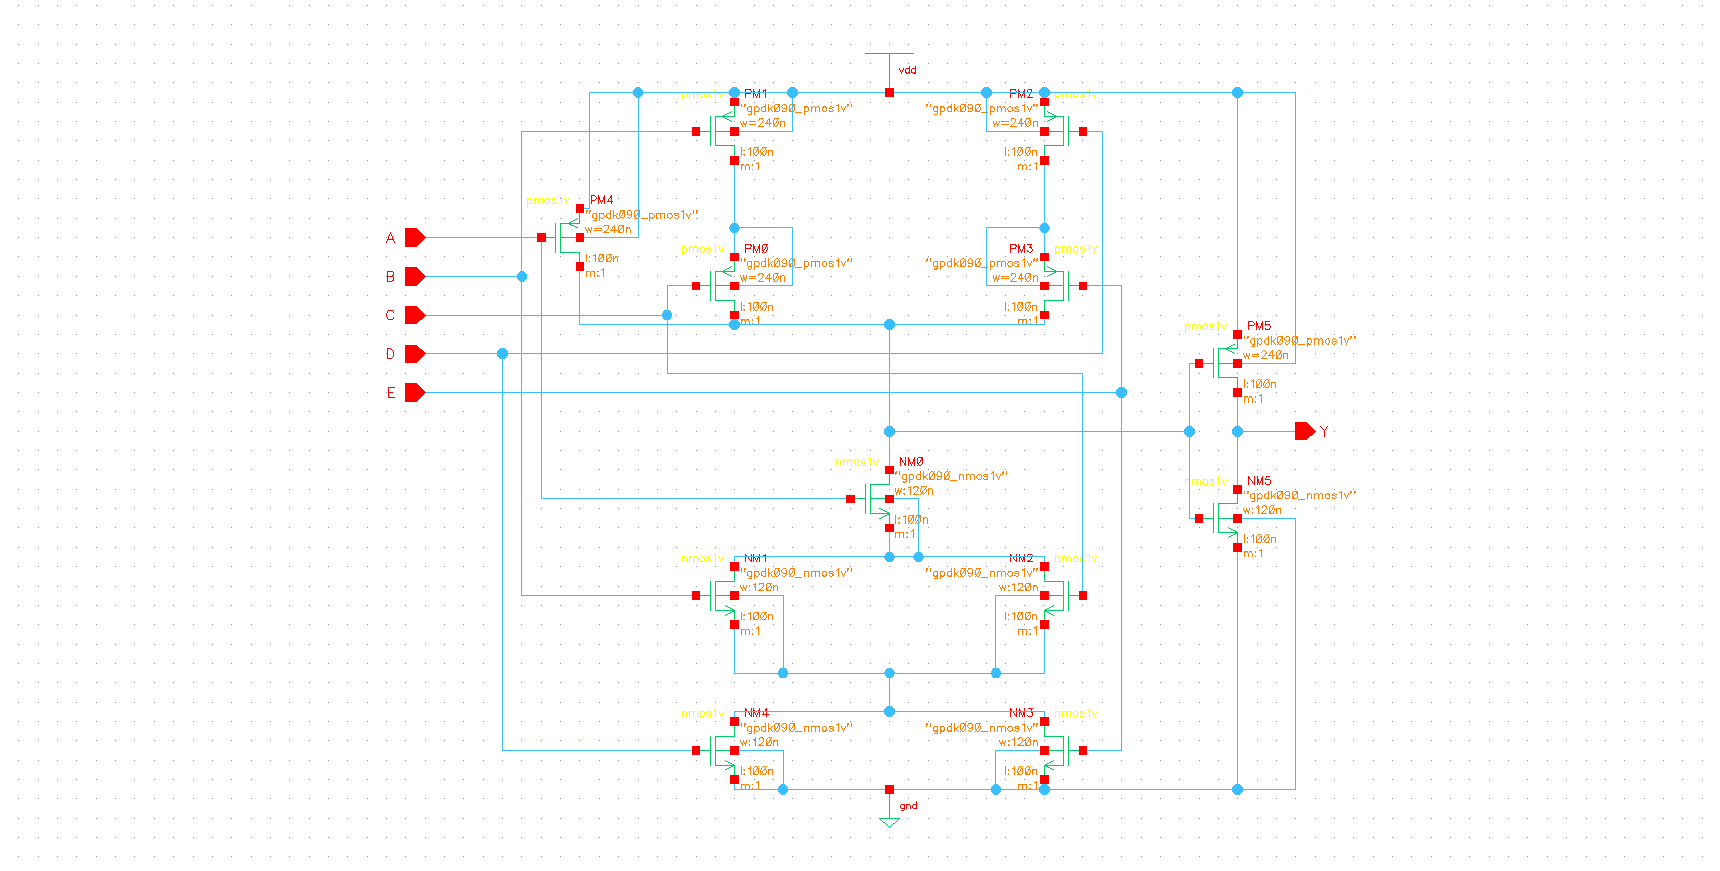
\includegraphics[width=\textwidth]{schematic.png}
    \caption{CMOS schematic diagram of the Boolean expression $Y=A\cdot(B+C)\cdot(D+E)$.}
\end{figure}
\begin{figure}[!h]
    \begin{subfigure}[h]{0.5\textwidth}
        \centering
        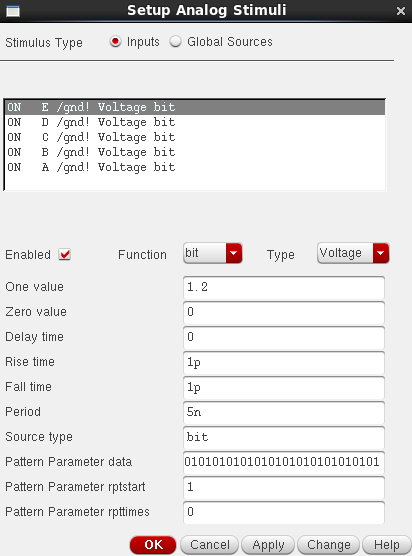
\includegraphics[width=0.95\textwidth]{e.png}
        \caption{Input Setup.}
    \end{subfigure}
    \begin{subfigure}[h]{0.5\textwidth}
        \centering
        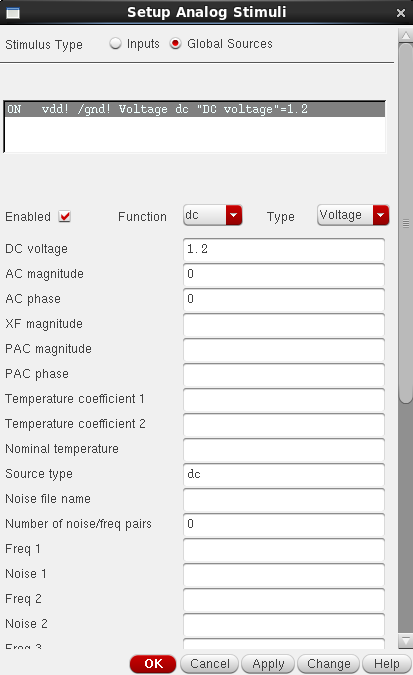
\includegraphics[width=0.95\textwidth,height=0.45\textheight]{global.png}
        \caption{Global source Setup.}
    \end{subfigure}
    \caption{Input and Global source Setup.}
\end{figure}
\newpage
\section{Simulation Result}
\begin{figure}[!h]
    \centering
    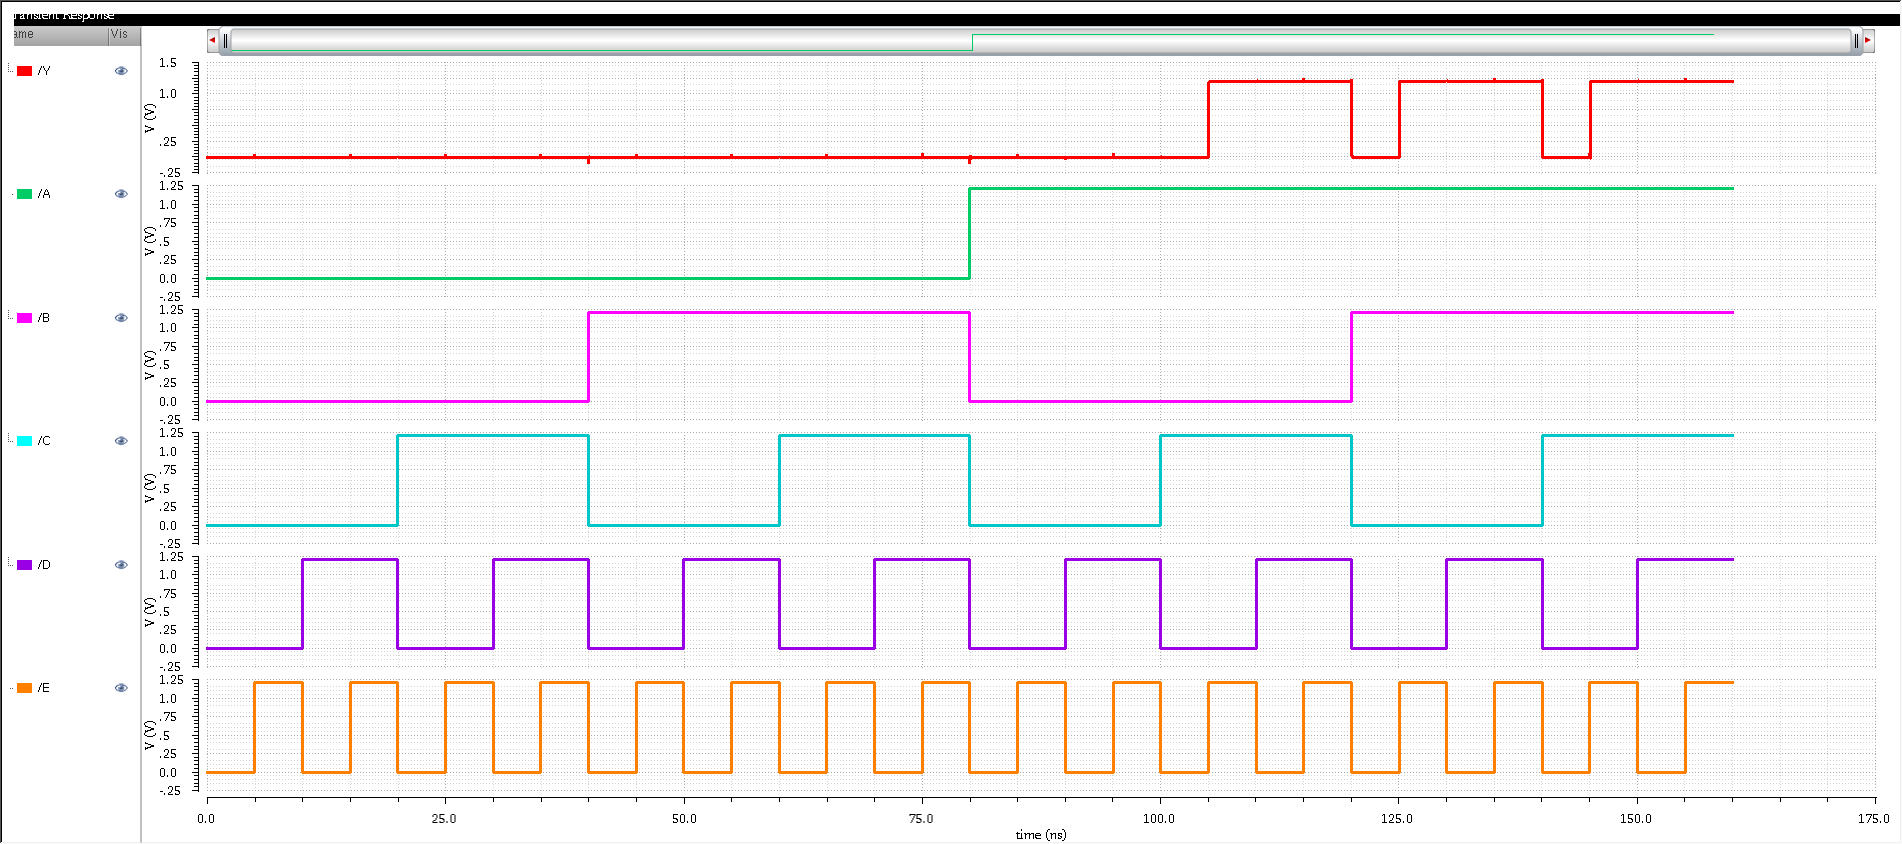
\includegraphics[width=\textwidth]{plot.png}
    \caption{Waveforms of inputs A (Green), B (Pink), C (Indigo), D (Purple), E (Orange) and output Y (Red).}
\end{figure}
\begin{longtable}[!h]{|l|l|l|l|l|c|}
    \hline
    $A$ & $B$ & $C$ & $D$ & $E$ & $Y=A\cdot(B+C)\cdot(D+E)$ \\ \hline
    0   & 0   & 0   & 0   & 0   & 0                         \\ \hline
    0   & 0   & 0   & 0   & 1   & 0                         \\ \hline
    0   & 0   & 0   & 1   & 0   & 0                         \\ \hline
    0   & 0   & 0   & 1   & 1   & 0                         \\ \hline
    0   & 0   & 1   & 0   & 0   & 0                         \\ \hline
    0   & 0   & 1   & 0   & 1   & 0                         \\ \hline
    0   & 0   & 1   & 1   & 0   & 0                         \\ \hline
    0   & 0   & 1   & 1   & 1   & 0                         \\ \hline
    0   & 1   & 0   & 0   & 0   & 0                         \\ \hline
    0   & 1   & 0   & 0   & 1   & 0                         \\ \hline
    0   & 1   & 0   & 1   & 0   & 0                         \\ \hline
    0   & 1   & 0   & 1   & 1   & 0                         \\ \hline
    0   & 1   & 1   & 0   & 0   & 0                         \\ \hline
    0   & 1   & 1   & 0   & 1   & 0                         \\ \hline
    0   & 1   & 1   & 1   & 0   & 0                         \\ \hline
    0   & 1   & 1   & 1   & 1   & 0                         \\ \hline
    1   & 0   & 0   & 0   & 0   & 0                         \\ \hline
    1   & 0   & 0   & 0   & 1   & 0                         \\ \hline
    1   & 0   & 0   & 1   & 0   & 0                         \\ \hline
    1   & 0   & 0   & 1   & 1   & 0                         \\ \hline
    1   & 0   & 1   & 0   & 0   & 0                         \\ \hline
    1   & 0   & 1   & 0   & 1   & 1                         \\ \hline
    1   & 0   & 1   & 1   & 0   & 1                         \\ \hline
    1   & 0   & 1   & 1   & 1   & 1                         \\ \hline
    1   & 1   & 0   & 0   & 0   & 0                         \\ \hline
    1   & 1   & 0   & 0   & 1   & 1                         \\ \hline
    1   & 1   & 0   & 1   & 0   & 1                         \\ 
    1   & 1   & 0   & 1   & 1   & 1                         \\ \hline
    1   & 1   & 1   & 0   & 0   & 0                         \\ \hline
    1   & 1   & 1   & 0   & 1   & 1                         \\ \hline
    1   & 1   & 1   & 1   & 0   & 1                         \\ \hline
    1   & 1   & 1   & 1   & 1   & 1                         \\ \hline
    \caption{Truth table based on the Simulation Result.}
\end{longtable}
\section{Conclusion}
The simulation of the CMOS schematic for the Boolean function $Y=A\cdot(B+C)\cdot(D+E)$ using Cadence Virtuoso successfully demonstrated the practicality of CMOS technology in digital logic design. The resulting circuit accurately represented the logical operations outlined in the Boolean equation, confirming the reliability of our design methodology. Through this lab, we gained valuable insights into the behavior of CMOS circuits, particularly in their response to different input combinations. The successful implementation underscored the importance of understanding both Boolean algebra and circuit design principles in the field of VLSI engineering.
\section{References}
\begin{enumerate}
    \item Lab Manual.
    \item Cadence Virtuoso Tutorial - University of Southern California.
\end{enumerate}
\end{document}